\chapter{Korrektur der Regler}
\label{ch:regler}

Mit der Bibliothek aus \cref{ch:bibliothek} liegt ein Stand vor, der sich exakt wie das
Altmodell verhält. In diesem Kapitel werden die Befunde B1 und B2 an den Reglern behoben.
Dazu werden die Regler zunächst nachvollziehbar neu ausgelegt
(\cref{sec:auslegung}) und die Korrekturen einzeln in der Simulation bewertet
(\cref{sec:p1b}). Die erste Bewertung erfüllte alle vorab festgelegten Kennzahlen, zeigte in
den Zeitverläufen aber eine Dauerschwingung. Deren Ursache lag nicht im Regler, sondern in der
Messkette des Simulationsmodells (\cref{sec:grenzzyklus}). Nach deren Korrektur zeigt
\cref{sec:p1b1} das Ergebnis.

% ---------------------------------------------------------------
\section{Reglerauslegung}
\label{sec:auslegung}

Die \ac{MA} berechnet die Reglerverstärkungen mit einer internen Funktion des Motor Control
Blockset (\texttt{mcb.internal.\allowbreak SetControllerParameters}). Sie ist von Matlab nicht dokumentiert, ihre Ergebnisse
hängen von den fehlerhaften Motordaten ab (B3) und ihre Ausgabe ist in einer Form, die im
Modell zum Fehler B1 geführt hat. Sie wird deshalb durch das Skript
\skript{foc\_design\_controllers} ersetzt, das die Auslegung mit Standardverfahren offenlegt
und die Strukturfelder des Altmodells füllt.

\subsection{Stromregler}

Die Strecke des Stromregelkreises einer Achse besteht aus der Statorwicklung
(Widerstand $R_s$, Induktivität $L$) und einer Ersatztotzeit $\sigma$, die Rechentotzeit
($1\,T_s$) und die mittlere Verzögerung der \ac{PWM} ($0{,}5\,T_s$) zusammenfasst:
\begin{equation}
  G_i(s) = \frac{1/R_s}{1 + s\,L/R_s} \cdot \frac{1}{1 + s\,\sigma},
  \qquad \sigma = 1{,}5\,T_s .
\end{equation}
Ausgelegt wird ein \ac{PI}-Regler $K_p\,(1 + 1/(s T_n))$ nach dem Betragsoptimum. Die
Nachstellzeit kompensiert die elektrische Zeitkonstante, die Verstärkung ergibt sich aus der
verbleibenden Totzeit:
\begin{equation}
  T_n = \frac{L}{R_s}, \qquad K_p = \frac{L}{2\sigma}, \qquad K_i = \frac{K_p}{T_n}.
\end{equation}
Der geschlossene Kreis hat dann eine Durchtrittsfrequenz von etwa
$f_c \approx 1/(2\pi \cdot 2\sigma)$. Da der Motor Oberflächenmagnete hat
($L_d = L_q$), sind $d$- und $q$-Regler gleich.

\subsection{Drehzahlregler}

Unter der Annahme, dass der Stromregelkreis gegenüber dem Drehzahlkreis schnell ist, reduziert
sich die Strecke auf das mechanische System mit Drehmomentkonstante $K_t = 1{,}5\,p\,\Psi$ und
Trägheitsmoment $J$:
\begin{equation}
  G_n(s) = \frac{K_t}{J\,s}.
\end{equation}
Die Verstärkung wird aus einer gewählten Durchtrittsfrequenz $\omega_c$ bestimmt, die
Nachstellzeit als Vielfaches von deren Kehrwert:
\begin{equation}
  K_p = \frac{J\,\omega_c}{K_t}, \qquad T_n = \frac{4}{\omega_c}.
\end{equation}
Der Faktor 4 ergibt ohne Berücksichtigung der Totzeiten eine Phasenreserve von etwa
\SI{76}{\degree}. Das Überschwingen auf einen
Sollwertsprung liegt wegen der Nullstelle des \ac{PI}-Reglers dennoch bei etwa
\SI{15}{\percent}. Gewählt ist $f_c = \SI{5}{\hertz}$. Die Bandbreite ist bewusst klein gewählt: Die
Drehzahl wird aus den Hall-Signalen gewonnen, die bei vier Polpaaren nur 24 Flanken je
Umdrehung liefern. Bei \SI{200}{\per\minute} liegen zwischen zwei Flanken
\SI{12,5}{\milli\second}, was wie eine zusätzliche Messtotzeit wirkt.

\subsection{Umrechnung in normierte Größen}

Das Modell rechnet in \ac{PU}. Die Verstärkungen müssen daher mit den Bezugsgrößen
umgerechnet werden, und zwar mit denen, die im Modell tatsächlich wirken. Wie Befund B4 zeigt,
sind das nicht die Werte aus der Struktur \texttt{PU\_System} der \ac{MA}. Die Bezugsgrößen
werden deshalb in \skript{foc\_pu\_system} aus der Signalkette abgeleitet:

\begin{itemize}
  \item \textbf{Strom:} Im Modell gilt $i_\mathrm{PU} = (\text{ADC} - \text{Offset})/2048$.
    Ein \ac{PU} ist der Strom, der den \ac{ADC} um 2048 Stufen aus dem Offset auslenkt.
    Mit der Messkette des \ac{EVM} (\cref{sec:p1b1}) ergibt sich
    \begin{equation}
      I_\mathrm{base} = \frac{2048 \cdot U_\mathrm{ref}/4095}{R_\mathrm{shunt} \cdot G_\mathrm{CSA}}
      = \frac{2048 \cdot \SI{3,36}{\volt}/4095}{\SI{3}{\milli\ohm} \cdot 10}
      \approx \SI{56,0}{\ampere}.
    \end{equation}
  \item \textbf{Spannung:} Die Raumzeigermodulation setzt eine normierte Stellgröße von 1 in
    die Strangspannung $U_\mathrm{dc}/\sqrt{3}$ um, also
    $U_\mathrm{base} = \SI{24}{\volt}/\sqrt{3} \approx \SI{13,86}{\volt}$.
\end{itemize}

Die normierte Stromreglerverstärkung ist dann
$K_{p,\mathrm{PU}} = K_{p,\mathrm{SI}} \cdot I_\mathrm{base}/U_\mathrm{base}$, die des
Drehzahlreglers $K_{p,\mathrm{PU}} = K_{p,\mathrm{SI}} \cdot \omega_\mathrm{base}/I_\mathrm{base}$.
\Cref{tab:auslegung} fasst die Ergebnisse für das Profil \texttt{datasheet} zusammen.
\skript{test\_config} prüft die Auslegung, indem es die Verstärkungen in SI-Einheiten
zurückrechnet und den Betrag des offenen Drehzahlkreises bei $f_c$ auswertet.

\begin{table}[htbp]
  \centering
  \caption{Ausgelegte Reglerparameter (Profil \texttt{datasheet},
    $T_s = \SI{50}{\micro\second}$, $T_{s,n} = \SI{0,5}{\milli\second}$)}
  \label{tab:auslegung}
  \small
  \begin{tabular}{@{}lrrr@{}}
    \toprule
    Größe & SI & \ac{PU} & Bemerkung \\
    \midrule
    \multicolumn{4}{@{}l}{\textit{Stromregler ($d$ und $q$)}} \\
    $K_p$ & \SI{0,253}{\volt\per\ampere} & \num{1,031} & $L/(2\sigma)$ \\
    $T_n$ & \SI{1,69}{\milli\second} & & $L/R_s$ \\
    $K_i$ & & \SI{606}{\per\second} & $K_p/T_n$ \\
    $f_c$ & \SI{1,06}{\kilo\hertz} & & $1/(2\pi\cdot 2\sigma)$ \\
    \midrule
    \multicolumn{4}{@{}l}{\textit{Drehzahlregler}} \\
    $K_p$ & \num{0,0053}\,A/min$^{-1}$ & \num{0,380} & $J\omega_c/K_t$ \\
    $T_n$ & \SI{127}{\milli\second} & & $4/\omega_c$ \\
    $K_i$ & & \SI{2,99}{\per\second} & $K_p/T_n$ \\
    $f_c$ & \SI{5}{\hertz} & & gewählt \\
    \bottomrule
  \end{tabular}
\end{table}

% ---------------------------------------------------------------
\section{Korrektur der Reglerblöcke (P1b)}
\label{sec:p1b}

\subsection{Änderungen}

Die Korrekturen werden von \skript{foc\_apply\_fixes} in der Bibliothek ausgeführt, getrennt
für Strom- und Drehzahlregler (\cref{tab:fixes}). Beide stellen die PID-Blöcke auf eine
Integralverstärkung in \si{\per\second} um (\texttt{UseKiTs = off}). Damit gibt es nur noch
eine Interpretation des Parameters, und die Ursache von B1 entfällt unabhängig davon, wie
\texttt{UseKiTs} im Altmodell gemeint war.

\begin{table}[htbp]
  \centering
  \caption{Korrekturen an den PID-Blöcken durch \skript{foc\_apply\_fixes}}
  \label{tab:fixes}
  \small
  \begin{tabularx}{\linewidth}{@{}l>{\raggedright\arraybackslash}X
      >{\raggedright\arraybackslash}X@{}}
    \toprule
    Parameter & vorher (Altmodell) & nachher \\
    \midrule
    \multicolumn{3}{@{}l}{\textit{Stromregler $d$, $q$ (\texttt{current\_pi}, B2)}} \\
    $P$ & \texttt{Kp\_i - 0.0002} & \texttt{Kp\_i} \\
    $I$ & \texttt{Ki\_texas*Ts}, \texttt{UseKiTs = on} & \texttt{Ki\_i} in \si{\per\second},
      \texttt{UseKiTs = off} \\
    Ausgang & $[0,\ 1]$ & $[-1,\ 1]$ \\
    \midrule
    \multicolumn{3}{@{}l}{\textit{Drehzahlregler (\texttt{speed\_pi}, B1)}} \\
    $I$ & \texttt{Ki\_speed\_texas*Ts\_speed}, \texttt{UseKiTs = on}
      & \texttt{Ki\_speed} in \si{\per\second}, \texttt{UseKiTs = off} \\
    Ausgang & $[-0{,}5,\ 1]$ & unverändert (später parametriert, \cref{ch:schutz}) \\
    \bottomrule
  \end{tabularx}
\end{table}

\subsection{Versuchsplan}

Das Skript \skript{foc\_run\_p1b} simuliert drei Läufe mit dem Profil \texttt{datasheet}
über \SI{8}{\second}: Lauf A mit den unkorrigierten Reglern, Lauf B nach der Korrektur der
Stromregler und Lauf C nach zusätzlicher Korrektur des Drehzahlreglers. Der Drehzahlsollwert
springt bei $t = \SI{1}{\second}$ von 0 auf \SI{0,25}{PU}, das Streckenmodell ist mit
\SI{10}{\percent} des Nennmoments belastet. Ausgewertet werden vier Kennzahlen über die letzten
\SI{20}{\percent} des Laufs:

\begin{itemize}
  \item $\bar e_n$: mittlere Drehzahlabweichung, zeigt eine bleibende Regelabweichung,
  \item $e_{iq,\mathrm{rms}}$, $e_{id,\mathrm{rms}}$: Effektivwert der Stromregelabweichung
    je Achse,
  \item $u_{d,\min}$: kleinste $d$-Spannung über den gesamten Lauf, zeigt, ob die
    Begrenzung auf $[0, 1]$ aufgehoben ist.
\end{itemize}

Die Erwartungen wurden vor den Läufen festgelegt: In Lauf A ist $u_{d,\min} \geq 0$ und
$\bar e_n \neq 0$; in Lauf B ist $e_{iq,\mathrm{rms}}$ deutlich kleiner als in A; in Lauf C
gilt zusätzlich $\bar e_n \approx 0$.

\subsection{Ergebnis}

\Cref{tab:p1b} zeigt die Kennzahlen. Formal ist jede Erwartung erfüllt. Die Zeitverläufe
in \cref{fig:p1b_e0} zeigen jedoch, dass in den Läufen B und C die $d$-Spannung ab etwa
\SI{0,05}{\second} fast rechteckförmig zwischen $\pm 0{,}9$ springt, mit etwa
\SI{325}{\hertz} und bis zum Ende des Laufs. Der Wert $u_{d,\min} = -0{,}94$ ist also die
Amplitude einer Dauerschwingung und kein Beleg für eine sinnvoll genutzte negative
Spannung. Der niedrige Wert von $e_{iq,\mathrm{rms}}$ ergibt sich, weil der Sollwert im
eingeschwungenen Zustand klein ist. Erst $e_{id,\mathrm{rms}} = 0{,}23$ zeigt die Schwingung.

\begin{table}[htbp]
  \centering
  \caption{Kennzahlen P1b (\SI{8}{\second}, Auswertung \SIrange{6,4}{8}{\second})}
  \label{tab:p1b}
  \small
  \begin{tabular}{@{}lrrrr@{}}
    \toprule
    Lauf & $\bar e_n$ & $e_{iq,\mathrm{rms}}$ & $e_{id,\mathrm{rms}}$ & $u_{d,\min}$ \\
    \midrule
    A unkorrigiert & \num{0,188} & \num{0,233} & \num{0,0097} & \num{0} \\
    B + Stromregler & \num{-0,0037} & \num{0,074} & \textbf{\num{0,235}} & \num{-0,943} \\
    C + Drehzahlregler & \num{-0,000004} & \num{0,073} & \textbf{\num{0,235}} & \num{-0,943} \\
    \bottomrule
  \end{tabular}
\end{table}

\begin{figure}[htbp]
  \centering
  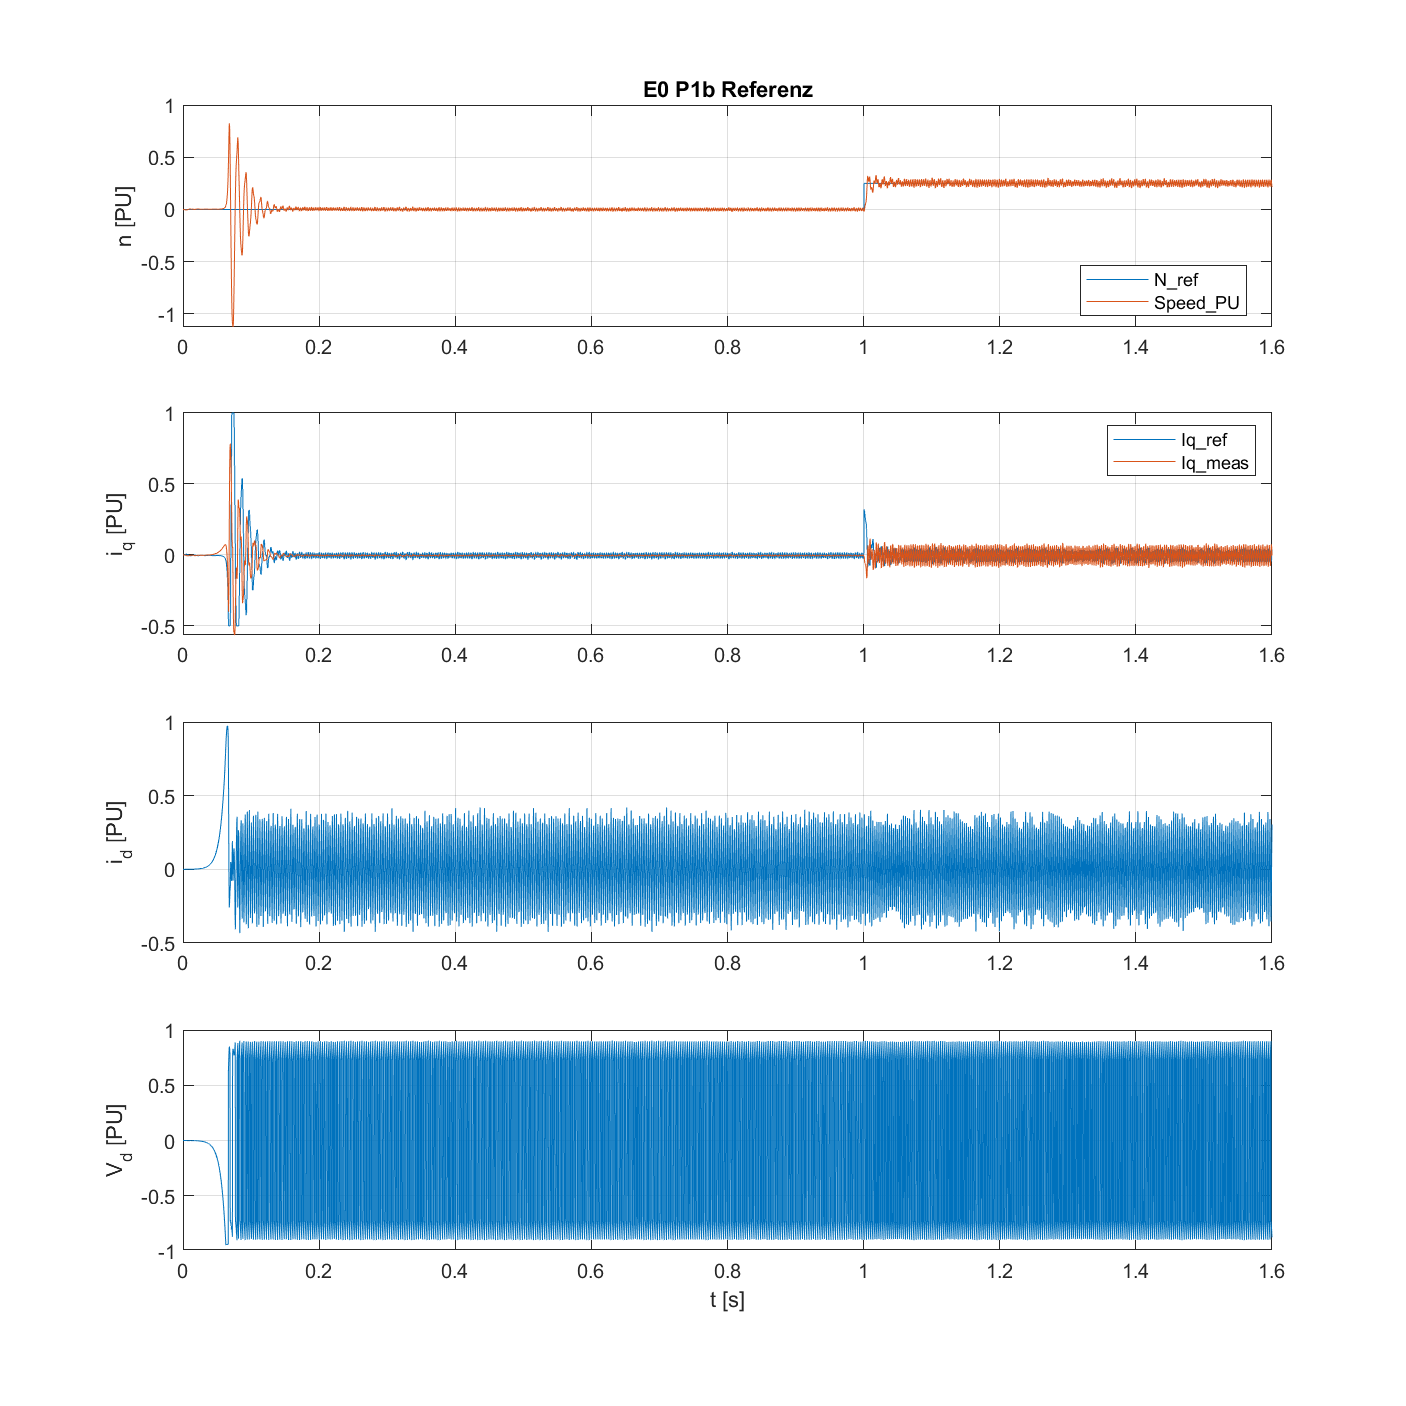
\includegraphics[width=0.9\linewidth]{P1b_diag_E0_P1b_Referenz}
  \caption{Stand P1b (korrigierte Regler, ursprüngliches Sensormodell): Drehzahl, $i_q$,
    $i_d$ und $u_d$ in \ac{PU}. Ab etwa \SI{0,05}{\second} schwingt der Stromregelkreis
    dauerhaft an der Stellgrößenbegrenzung.}
  \label{fig:p1b_e0}
\end{figure}

Der Stand wurde als \texttt{P1b} getaggt, um den Befund reproduzierbar zu halten, aber nicht
als hardwaretauglich freigegeben. Seitdem gehört zur Bewertung jedes Laufs die Sichtprüfung
der Zeitverläufe, insbesondere von $u_d$ und $i_d$.

% ---------------------------------------------------------------
\section{Diagnose des Grenzzyklus}
\label{sec:grenzzyklus}

Die Schwingung wurde nicht durch Nachstellen der Reglerparameter behandelt, sondern zunächst
rein lesend untersucht. Logging-Einstellungen wurden nur im Arbeitsspeicher gesetzt, die
Modelle nach jedem Lauf ohne Speichern geschlossen.

\subsection{Vorzeichen des Regelkreises}

Aus einer Simulation wurden die $d/q$-Größen aus Sicht des Reglers ($C$) und die
$d/q$-Größen der Strecke ($P$, Signale des Motorblocks) aufgezeichnet und per komplexer
Regression ins Verhältnis gesetzt:

\begin{itemize}
  \item Strompfad: $\underline{I}_C = k \cdot \underline{I}_P$ mit
    $|k| = \SI{560}{\ampere}/\mathrm{PU}$ und einer Drehung von \SI{-172,7}{\degree},
  \item Spannungspfad: $\underline{U}_C = k \cdot \underline{U}_P$ mit
    $|k| = \SI{14,7}{\volt}/\mathrm{PU}$ und einer Drehung von \SI{+7,2}{\degree}.
\end{itemize}

Ein reiner Fehler im Rotorwinkel würde beide Pfade um denselben Winkel mit
entgegengesetztem Vorzeichen drehen und sich im Kreis aufheben. Hier liegen die Drehungen
aber \SI{180}{\degree} auseinander. Wirksam ist damit $\underline{I}_C \approx -G \cdot
\underline{U}_C$: Der Stromregelkreis ist \textbf{mitgekoppelt}. Die Gegenprobe über das
Drehmoment bestätigt das: Ein positives $i_q$ aus Sicht des Reglers erzeugt ein negatives
Moment, betragsmäßig passend zur Drehmomentkonstante.

Die Mitkopplung treibt die Regler an ihre Grenze. Die Strecke erhält dann
$\pm\SI{12,5}{\volt}$ an \SI{22,5}{\milli\ohm}, die Ströme steigen bis über \SI{500}{\ampere},
bis der simulierte Stromsensor sättigt. Ohne Rückführung läuft der Integrator voll, und es
entsteht ein Kippschwingen zwischen Stellgrößen- und Sensorbegrenzung. Im Altmodell fiel das
nicht auf, weil die Begrenzung auf $[0, 1]$ und der verschwindend kleine Integralanteil ein
Weglaufen verhinderten. Die Korrektur der Regler hat die Mitkopplung also nicht verursacht,
sondern sichtbar gemacht.

\subsection{Experimente zur Bestätigung}

Um die Ursache einzugrenzen, wurden drei Varianten nur im Arbeitsspeicher simuliert
(\cref{tab:diag}). Eine Drehung des Rotorwinkels um \SI{180}{\degree} (E1) kehrt nur das
Momentvorzeichen um, der Kreis bleibt mitgekoppelt. Eine Invertierung der Strommessung (E2)
beseitigt die Schwingung vollständig. Wird zusätzlich die Auslegung auf die im
Simulationspfad wirksame Bezugsgröße angepasst (E3), folgt der Iststrom dem Sollwert nahezu
deckungsgleich.

\begin{table}[htbp]
  \centering
  \caption{Diagnoseexperimente (nur im Arbeitsspeicher, \SI{1,6}{\second},
    Auswertung \SIrange{1,28}{1,6}{\second})}
  \label{tab:diag}
  \small
  \begin{tabularx}{\linewidth}{@{}l>{\raggedright\arraybackslash}Xrrr@{}}
    \toprule
    & Änderung & $\mathrm{std}(u_d)$ & $e_{id,\mathrm{rms}}$ & $\max |i|$ \\
    \midrule
    E0 & keine (Stand P1b) & \num{0,810} & \num{0,231} & \SI{532}{\ampere} \\
    E1 & Rotorwinkel $+\SI{180}{\degree}$ & \num{0,685} & \num{0,321} & \SI{517}{\ampere} \\
    E2 & Strommessung invertiert & \num{0,0001} & \num{0,0003} & \SI{36}{\ampere} \\
    E3 & wie E2, Regler auf wirksame Bezugsgröße & \num{0,0018} & \num{0,0002} & \SI{7,5}{\ampere} \\
    \bottomrule
  \end{tabularx}
\end{table}

\subsection{Ursache: Polarität der Strommessung}

Ob die Invertierung der Strommessung der richtige Ort der Korrektur ist, lässt sich nur
an der realen Hardware entscheiden. Die Unterlagen des \ac{EVM} wurden deshalb ausgewertet.
Das Benutzerhandbuch \cite{ti_slvubv6} nennt Shunt (\SI{3}{\milli\ohm}), Verstärkung
(\SI{10}{\volt\per\volt}) und Offset (\SI{1,65}{\volt}), aber nicht die Polarität. Aus der
Netzliste des Schaltplans \cite{ti_slvc817} folgt: Der Strommessverstärker ist ein
Differenzverstärker mit $G = \SI{49,9}{\kilo\ohm}/(\SI{4,99}{\kilo\ohm} + \SI{10,2}{\ohm})
= \SI{9,98}{\volt\per\volt}$, dessen nicht invertierender Eingang an der FET-Seite des Shunts
liegt. Damit gilt
\begin{equation}
  U_\mathrm{ISEN} = \SI{1,65}{\volt} + \SI{29,9}{\milli\volt\per\ampere} \cdot I_{\mathrm{Shunt}\downarrow},
\end{equation}
wobei $I_{\mathrm{Shunt}\downarrow}$ von der FET-Source nach Masse fließt. Ein Strom, der in
den Motor fließt, kommt während der Low-Side-Leitphase von Masse durch den Shunt nach oben.
\textbf{Ein positiver Strangstrom ergibt also einen \ac{ADC}-Wert unter \SI{1,65}{\volt}.}

Das Sensormodell der Simulation bildete diese Umkehr nicht ab. Es enthielt außerdem nur den
Shunt, nicht die Verstärkung, und lag damit um den Faktor 10 neben der Hardware. Auf der
Spannungsseite enthalten Simulation und Code dagegen dieselbe Umkehr: Der Block
\block{Scaling DutyCycles} berechnet in beiden Varianten $0{,}5 - 0{,}5\,x$. Die \ac{MA}
erklärt diese Negation mit unterschiedlichen Drehrichtungskonventionen. Nach diesem Befund
kompensiert sie tatsächlich die invertierende Strommessung des \ac{EVM}
(\cref{tab:vorzeichen}).

\begin{table}[htbp]
  \centering
  \caption{Vorzeichen im Stromregelkreis}
  \label{tab:vorzeichen}
  \small
  \begin{tabular}{@{}lcccc@{}}
    \toprule
    & Spannungsseite & Strecke & Strommessung & Kreis \\
    \midrule
    Simulation (P1b) & $-1$ & $+1$ & $+1$ & mitgekoppelt \\
    Hardware (\ac{EVM}) & $-1$ & $+1$ & $-1$ & gegengekoppelt \\
    Simulation (P1b.1) & $-1$ & $+1$ & $-1$ & gegengekoppelt \\
    \bottomrule
  \end{tabular}
\end{table}

Der Grenzzyklus ist damit ein Fehler des Simulationsmodells, nicht der Regler und nicht des
Codegenerierungspfads. Das erklärt auch, warum die Firmware der \ac{MA} auf der Hardware lief,
obwohl ihr Simulationspfad mitgekoppelt war.

% ---------------------------------------------------------------
\section{Ergebnis mit korrigierter Messkette (P1b.1)}
\label{sec:p1b1}

\subsection{Änderungen}

Die Korrektur erfolgte in drei einzelnen Schritten, jeder mit eigenem Commit und Nachweis:

\begin{enumerate}
  \item \textbf{Messkette in der Konfiguration:} In \skript{foc\_cfg\_inverter\_drv8300}
    werden die Steigung auf $\SI{3}{\milli\ohm} \cdot 10 = \SI{0,03}{\volt\per\ampere}$, der
    Messbereich auf \SI{55}{\ampere} und die Polarität auf \texttt{invertingAmp = -1} gesetzt.
    Nachweis: \skript{test\_config}.
  \item \textbf{Bezugsgrößen:} \skript{foc\_pu\_system} leitet $I_\mathrm{base}$ und
    $U_\mathrm{base}$ aus der Signalkette ab (\cref{sec:auslegung}). Die Verstärkungen in SI
    bleiben unverändert, nur ihre Darstellung in \ac{PU} ändert sich. Nachweis:
    \skript{test\_config}.
  \item \textbf{Sensormodell:} Ausgehend vom Stand P1a setzt \skript{foc\_fix\_sim\_sensor}
    die Verstärkung im Sensormodell der Strecke auf
    \texttt{invertingAmp*ISenseVoltPerAmp}. Das betrifft nur den Simulationspfad. Mit dem
    Profil \texttt{legacy\_f2838}, das die alten Werte enthält, bleibt das Modell bitgleich.
    Nachweis: \skript{foc\_check\_equivalence}, alle Abweichungen null.
\end{enumerate}

Der Codegenerierungspfad bleibt unverändert, da die Hardware bereits richtig gegengekoppelt
ist. Anschließend wurden die Läufe A, B und C mit denselben Korrekturen wie in P1b wiederholt.

\subsection{Ergebnis}

\Cref{tab:p1b1} zeigt die Kennzahlen, \cref{fig:p1b1} die Zeitverläufe von Lauf C.

\begin{table}[htbp]
  \centering
  \caption{Kennzahlen P1b.1 (\SI{8}{\second}, Auswertung \SIrange{6,4}{8}{\second})}
  \label{tab:p1b1}
  \small
  \begin{tabular}{@{}lrrrr@{}}
    \toprule
    Lauf & $\bar e_n$ & $e_{iq,\mathrm{rms}}$ & $e_{id,\mathrm{rms}}$ & $u_{d,\min}$ \\
    \midrule
    A unkorrigiert & \num{0,213} & \num{0,030} & \num{0,043} & \num{0} \\
    B + Stromregler & \num{0,118} & \num{0,00018} & \num{0,00020} & \num{-0,015} \\
    C + Drehzahlregler & \num{0,0000005} & \num{0,00017} & \num{0,00017} & \num{-0,036} \\
    \bottomrule
  \end{tabular}
\end{table}

\begin{figure}[htbp]
  \centering
  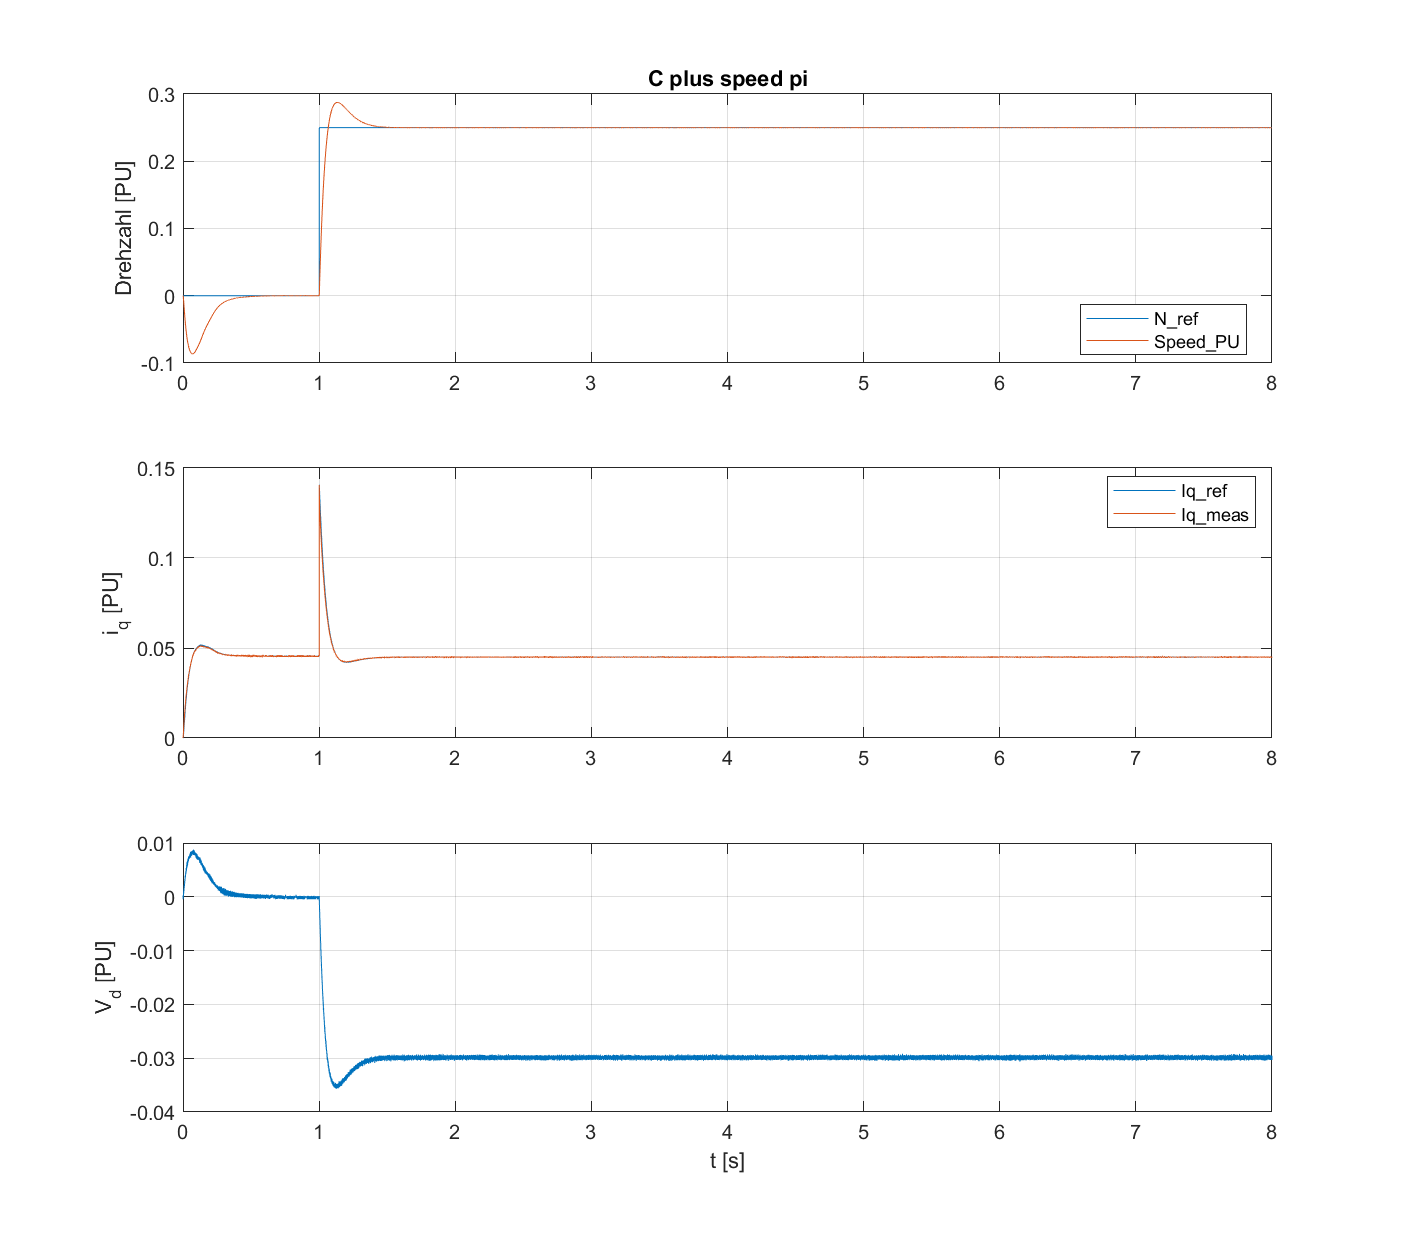
\includegraphics[width=0.9\linewidth]{P1b_C_plus_speed_pi}
  \caption{Stand P1b.1, Lauf C (Strom- und Drehzahlregler korrigiert): Drehzahl, $i_q$ und
    $u_d$ in \ac{PU} bei einem Sollwertsprung auf \SI{0,25}{PU} bei $t = \SI{1}{\second}$
    und \SI{10}{\percent} Lastmoment}
  \label{fig:p1b1}
\end{figure}

Die Ergebnisse sind auch physikalisch plausibel:

\begin{itemize}
  \item \textbf{Lauf A:} Der unkorrigierte Stromregler kann keine negative $d$-Spannung
    stellen, und sein Integralanteil ist praktisch wirkungslos. Der Iststrom bleibt unter dem
    Sollwert, die Drehzahl erreicht nur etwa \SI{0,04}{PU} statt \SI{0,25}{PU}.
  \item \textbf{Lauf B:} Der Iststrom folgt dem Sollwert deckungsgleich. Die bleibende
    Drehzahlabweichung entspricht genau dem P-Verhalten des noch unkorrigierten
    Drehzahlreglers: $i_{q,\mathrm{Last}}/K_p = 0{,}045/0{,}380 = 0{,}118$.
  \item \textbf{Lauf C:} Die Drehzahl folgt dem Sprung mit etwa \SI{15}{\percent}
    Überschwingen und ist nach etwa \SI{0,5}{\second} eingeschwungen, wie für
    $f_c = \SI{5}{\hertz}$ und $T_n = 4/\omega_c$ erwartet. Die anfängliche Abweichung auf
    \SI{-0,09}{PU} entsteht, weil das Lastmoment bereits während der Offsetkalibrierung wirkt,
    in der die Regelung noch nicht arbeitet.
  \item \textbf{$d$-Spannung:} $u_d$ wird mit steigender Drehzahl negativ ($-0{,}015$ bei
    \SI{0,13}{PU}, $-0{,}030$ bei \SI{0,25}{PU}), wie es die Verkopplung
    $u_d \approx -\omega L i_q$ verlangt.
\end{itemize}

Damit erfüllt der Stand P1b.1 die Erwartungen sowohl in den Kennzahlen als auch in den
Zeitverläufen. Er wurde mit dem Tag \texttt{P1b.1} versehen und bildet die Grundlage für die
folgenden Kapitel.

Für die Inbetriebnahme auf der Hardware bleiben zwei Punkte zu beachten. Erstens ist das
Vorzeichen der Strommessung aus dem Schaltplan abgeleitet und sollte vor dem ersten geregelten
Lauf gemessen werden: Ein kleiner Gleichstrom in Phase A muss einen negativen Wert von
$i_{a,\mathrm{PU}}$ ergeben. Zweitens erlaubt die Untergrenze des Drehzahlreglers von $-0{,}5$
ein Bremsen, dessen Energie ein Labornetzteil nicht aufnehmen kann. Beide Punkte werden in
\cref{ch:codegen} und \cref{ch:schutz} behandelt.

\offen{Ergebnis der Vorzeichenmessung auf der Hardware ergänzen bzw.\ auf Hardwareteil verweisen}
